\subsubsection{Módulos de temperatura del habitáculo}

Para automatizar el climatizardor en un futuro, necesitamos poder conocer la temperatura, con cierta precisión, en
el interior del vehículo. Actualmente disponemos de varios sensores en el mercado que nos permiten medir la 
temperatura pero, todos disponen de un margen de error que se arrastra en cada lectura. Con el fin de reducir
el error del sensor, se plantea dividir el habitáculo del vehículo en 4 cuadrantes de forma que dispongamos
de un sensor por cada cuadrante.

\begin{figure}[H]
    \centering
    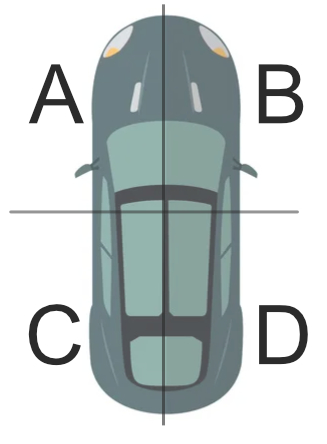
\includegraphics[width=4cm]{figures/clima-cuadran.jpg}
    \caption{Diagrama de los cuadrantes del vehículo.}
    \label{fig:climatización_cuadrantes}
\end{figure}

Mediante la división en cuadrantes tendremos a nuestra disposición 4 mediciones con las
que podremos realizar una media ponderada que será la medición más cercana a la realidad.\\

Esta media de mediciones se nos hace obligada, en parte, por la definición de temperatura, pues no es más que
la energía cinética de un sistema termodinámico, medición que sufre severas alteraciones debido a cualquier 
radiación directa de infrarojos.\textit{(Esto se puede observar si el sensor se deja al sol directo, la temperatura 
se disparará pero no será la temperatura del sistema termodinámico que es el habitáculo)}.

\subsubsection*{Componentes}

Para el desarrollo de los sensores de temperatura usaremos un sensor de grado médico para disponer de mayor precisión,
el \textbf{TMP117} en su empaquetado SMD. Este sensor nos permite una comunicación $I^2C$ y una precisión de 0,10 ºC,
lo que nos resulta atractivo para poder precisar la temperatura ambiente. \\

Como cerebro del sistema, durante las pruebas, se plantea usar un \textbf{Atmega 328P}, un microcontrolador de 8 
bits con soporte para reloj de hasta 16 MHz.

Para el producto final se plantea optimizar el diseño y reducir costes usando un \textbf{AtTiny87} que nos permite
usar tanto $I^2C$ como \textit{ISP} para la comunicación entre sensor y transreceptor CAN.


\subsubsection*{Diagrama del circuito}

\includepdf[pages={2}]{figures/TP-0010U001.pdf}
